\section{Introduction}

%AVs must be safe
Autonomous vehicles are considered to be one of the most challenging types of reactive systems currently under 
development~\cite{AlurMT16, WongpiromsarnKF11, RamanDSMS15}. 
They need to interact reliably with a highly reactive environment and crashes cannot be tolerated.
Life critical decisions have to be made instantaneously and need to be executed at the right point in time. 
However, even if the intricate task of designing such systems is conquered, that the result must be guaranteed to be also safe and reliable.

%static program analysis can help
To ensure that such systems are indeed safe, there has been much work in static program analysis.
One major advancement from the programming languages community towards bug-free software has been the development of functional languages.
Functional languages use language features to control the space of possible programs via abstraction, which can prevent many common programming errors.

%a good 'static analysis' tool is to use a functional language
One static analysis tool that has proved useful is a strong type system as featured in functional languages~\cite{cardelli1996type}.
Another example is functional purity, which reduces the possibility of malformed state that can cause unexpected behavior.
In the simplest case, the higher-order function \texttt{map} common to functional languages is an abstraction for looping (among other functions) that eliminates the typical intermediate counter.
This helps to eliminate the possibility for runtime index out of bounds errors due to mistaken reasoning about edge cases.

%as an example, look at hardware and low level code
Because of these saftey benefits, functional languages are now also used for critical systems such as hardware.
ClaSH was used to program an FPGA to solve N Queens in a purely functional language~\cite{clash2014}.
FPGA programs can be difficult because of the low level memory and instruction management, but functional languages can abstract some of these issues away from the user.
Another example is Ivory, a functional language that compiles directly to C code that was used to build safer autonomous vehicles~\cite{pike2014}
This language still provides access to the low level operations necessary for embedded system programming, but still enforces good programming practice, such as disallowing pointer arithmetic, with a rich type system.
%TODO include ref to {Kansas Lava}

%when applying FP to reactive systems purity is hard
However, despite these advantages of functional programming, there are some difficulties when applying this approach to reactive systems.
One difficulty with can be the insistence on purity, which separates data manipulation code from sources of unknown data, such as IO.
Since reactive systems require a constant interaction between the environment and the agent, purity is sometimes seen as an obstacle.

%also there are many types of time
Furthermore, reactive systems require a consistent notion of time, communication, and actions.
For example, it is sometimes necessary to control a vehicle as an isolated agent, but it is also desirable to platoon a group a vehicles.
This requires opening communication channels between vehicles, introducing the rate of sensing and a rate of communication.
There may also be a need to have both continuous and discrete time behaviors.
In a car, the steering wheel should act as a continuous signal, but a human-in-the-loop system~\cite{li2014synthesis} should additionally respond to discrete user actions, such as turning on a directional.
Functional Reactive Programming achieves this by creating an abstraction of time on the type level that allows for both continuous and discrete behaviors.
%TODO  motivate on some example (synchronous vs asynchronous, real vs discrete),

%but FRP can help us
A solution to this problem is to use a paradigm called Functional Reactive Programming (FRP)~\cite{hudak2003arrows,hudak2000haskell}.
FRP uses abstractions of computations available in functional languages (\eg monads, arrows, applicatives) to allow for a separation between environment handling and computation.
This separation makes functional languages powerful in a number of different reactive settings.
In fact, the ability to separate types of computations can also be helpful in building reactive system that are easily analyzed.

%What did we do?
We have built a library, \ourLib, to use FRP to control a vehicle inside a simulation.
In the sequel, we will demonstrate the flexibility of this library.
In addition to single vehicle control, \ourLib allows for easy simulation on open communication channels between vehicles.
This is a critical component of modern autonomous vehicle research, especially towards the goal of safe platooning algorithms~\cite{?}.
As we will show, using \ourLib provides a simple interface for simulating this communication, which can ease the development task for testing novel algorithms in this domain.

%we will explain FRP in depth in the sequel
In summary, we make the following contributions:

\begin{itemize}
\item An introduction to Functional Reactive Programming (FRP) using a simple reactive vehicle controller. We describe how FRP it allows for easier reasoning about correctness properties in reactive systems.
%\cfelix{this is the most important part, almost sure that nobody of the reviews will know about; go through the very basics, remember these are embedded systems people}

\item A library, \ourLib, for connecting Haskell to The Open Racing Car Simulator (TORCS), encouraging further research into the use of functional languages for the development of safer autonomous vehicle controllers. This library additionally supports communication between vehicle controllers, allows for research into platooning strategies.

\item A demonstration of an FRP controller for a vehicle that highlights the elegance and simplicity of the framework,
   which makes it resistant against errors. Furthermore it is easily extendable without breaking the remaining system.

\end{itemize}

\begin{figure}[t]
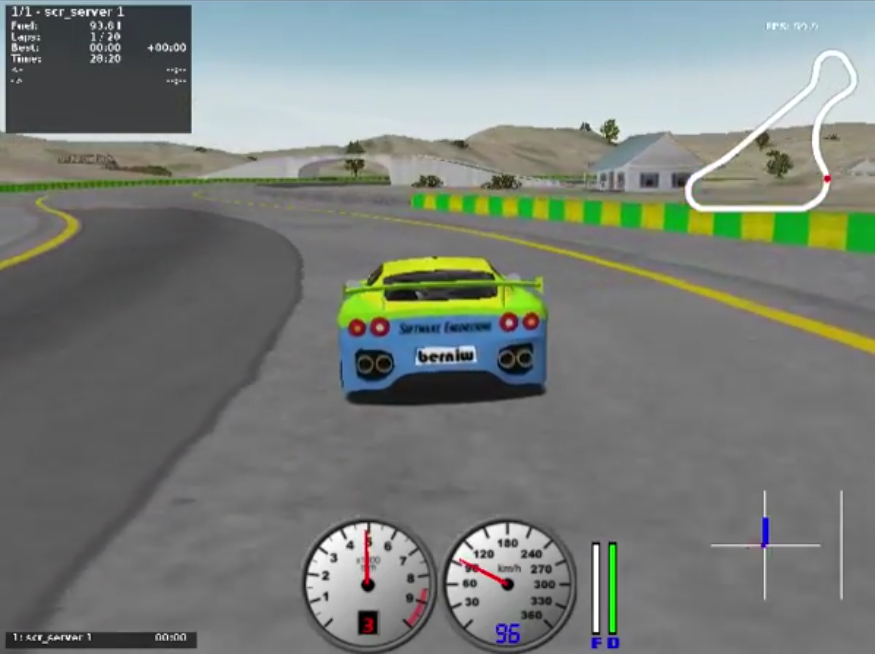
\includegraphics[width=0.45\textwidth]{figs/racing.png}
\caption{A screenshot of Haskell controlling the autonomous vehicle in the TORCS simulator}
\label{fig:race}
\end{figure}
